\section{Bewegungsplanung}

\textbf{Ziel}: Erzeugen einer kollisionsfreien Trajektorie unter Berücksichtigung verschiedener Ziele und Einschränkungen

\textbf{Arbeits- und Konfigurationsraum}:
\begin{itemize}
	\item \textbf{Arbeitsraum} $W$: Kartesischer Raum $\R^6$, in dem sich der \textbf{Tool Center Point} (TCP) aufhalten kann
	\item \textbf{Konfiguration} $\mathbf{q}\in C$ beschreibt den Zustand eines Roboters als Gelenkwinkelvektor im Gelenkwinkelraum
	\item \textbf{Konfigurationsraum} $C=C_\text{free}\cup C_\text{obs}\,$: $n$-dimensionaler Raum aller Gelenkwinkelkonfigurationen
	\item \textbf{Freiraum} $C_\text{free}=C\setminus C_\text{obs}\,$: Alle kollisionsfreie Konfigurationen. Für komplexere Kinematiken kann $C_\text{free}$ nicht effizient berechnet werden $\rightarrow$ Verwendung approximativer Verfahren
	\item \textbf{Hindernisraum} $C_\text{obs}$: Alle Konfigurationen, die zur einer Kollision führen
	\item $C_\text{free}$ und $C_\text{obs}$ ändern sich während der Ausführung
\end{itemize}

\textbf{Bewegungsplanung - Begrifflichkeiten}:
\begin{itemize}
	\item \textbf{Vollständiger Algorithmus}: Findet für ein Problem mindestens eine Lösung oder erkennt in endlicher Zeit, dass keine Lösung existiert
	\item \textbf{Randomisierter Algorithmus}: Verwenden Zufallsgrößen, um den Ablauf zu steuern, wobei oft heuristische Annahmen genutzt werden, um die Berechnung zu beschleunigen
	\item \textbf{Auflösungsvollständiger Algorithmus}: Approximativer Algorithmus, der zusätzlich vollständig ist
	\item \textbf{Probabilistisch-vollständiger Algorithmus}: Findet mindestens eine Lösung falls sie existiert, aber kann nicht erkennen, dass keine Lösung existiert
	\item Allgemeine Bewegungsplanungsaufgaben sind \textbf{PSPACE-vollständig}
\end{itemize}
\bigskip
\textbf{Problemklassen der Bewegungsplanung}:
\begin{itemize}
	\item \textbf{Klasse a}:
	\begin{itemize}
		\item \textbf{Gegeben}: Vollständiges Weltmodell, vollständige Nebenbedingungen
		\item \textbf{Gesucht}: Kollisionsfreie Trajektorie vom Start- zum Zielzustand 
	\end{itemize}
	\item \textbf{Klasse b}:
	\begin{itemize}
		\item \textbf{Gegeben}: Unvollständiges Weltmodell, unvollständige Nebenbedingungen
		\item \textbf{Gesucht}: Kollisionsfreie Trajektorie vom Start- zum Zielzustand 
		\item \textbf{Problem}: Kollision mit unbekannten Objekten 
	\end{itemize}
	\item \textbf{Klasse c}:
	\begin{itemize}
		\item \textbf{Gegeben}: Zeitvariantes Weltmodell (bewegliche Hindernisse)
		\item \textbf{Gesucht}: Kollisionsfreie Trajektorie vom Start- zum Zielzustand
		\item \textbf{Problem}: Hindernisse in Ort und Zeit variant
	\end{itemize}
	\item \textbf{Klasse d}:
	\begin{itemize}
		\item \textbf{Gegeben}: Zeitvariantes Weltmodell
		\item \textbf{Gesucht}: Trajektorie zu einem beweglichen Ziel
		\item \textbf{Problem}: Zielzustand in Ort und Zeit beweglich 
	\end{itemize}
	\item \textbf{Klasse e}:
	\begin{itemize}
		\item \textbf{Gegeben}: Kein Weltmodell $\rightarrow$ Muss erst erzeugt werden
		\item \textbf{Gesucht}: Kollisionsfreie Trajektorie vom Start- zum Zielzustand
	\end{itemize}
\end{itemize}

\textbf{Ansatz für die Pfadplanung für mobile Roboter}:
\begin{enumerate}
	\item Konstruiere ein Wegenetz $W$ in $C_\text{free}$
	\item Bilde $\mathbf{q}_\text{Start}$ und $\mathbf{q}_\text{Ziel}$ auf die nächsten Knoten $\mathbf{q'}_\text{Start}$ und $\mathbf{q'}_\text{Ziel}$ in $W$ ab
	\item Suche in $W$ einen Weg von $\mathbf{q'}_\text{Start}$ nach $\mathbf{q'}_\text{Ziel}$
	\item Finde einen Weg zwischen $\mathbf{q}_\text{Start}$ und  $\mathbf{q'}_\text{Start}$, sowie zwischen $\mathbf{q'}_\text{Ziel}$ und $\mathbf{q}_\text{Ziel}$
	\begin{center}
		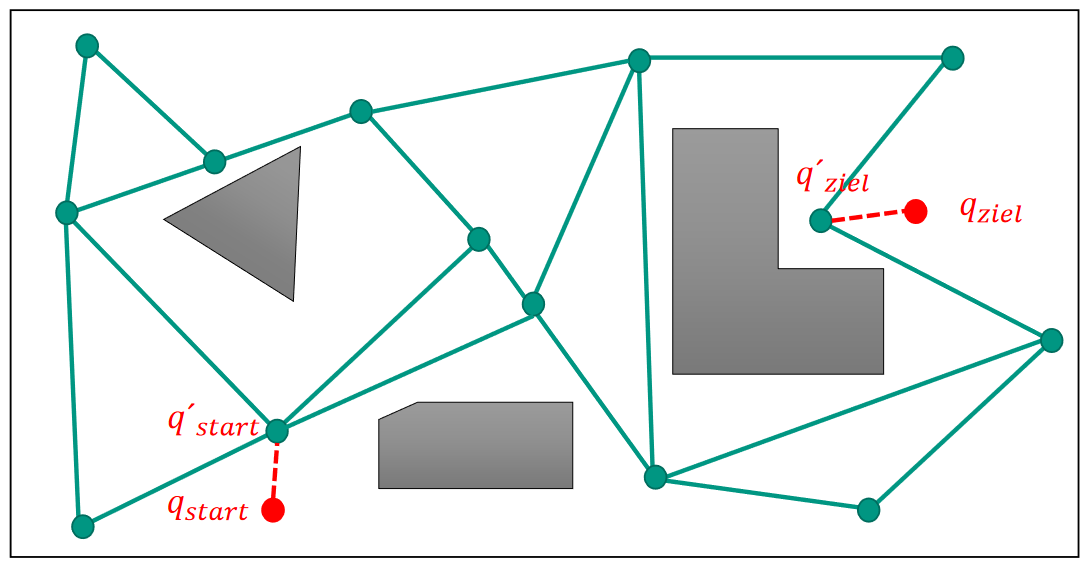
\includegraphics[width=0.6\textwidth]{images/pfadplanung.png}
	\end{center}
\end{enumerate}

\textbf{Konstruktion des Wegenetzes} $W$ durch Voronoi-Diagramme, Sichtgraphen oder  Zellzerlegung.

\textbf{Suche im Wegenetz} durch Baumsuche oder $A^*$-Algorithmus\\

\textbf{Voronoi-Diagramme}: 
\begin{itemize}
	\item Region des Voronoi-Diagramms ist definiert als die Menge aller Punkte, deren Abstand zum Hindernis geringer ist als zu allen anderen Hindernissen
	\item Punkte auf der Grenze zwischen zwei Regionen des Voronoi-Diagramms besitzen den gleichen Abstand zum eigenen und zum benachbarten Hindernis
	\begin{center}
		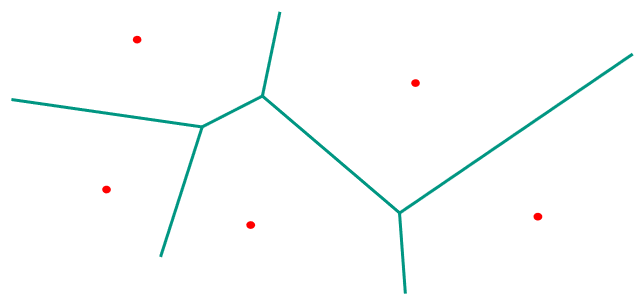
\includegraphics[width=0.4\textwidth]{images/voronoi.png}
	\end{center}
	\item \textbf{Konstruktion} mit Mittelsenkrechten, s. \textit{7/33-39}
	\item \textbf{Vorteile}: Maximaler Abstand zu Hindernissen
	\item \textbf{Nachteile}: In der Regel ist der gefunden Weg nicht der kürzeste. Bei wenigen Hindernissen werden nur wenige Wege generiert
\end{itemize}
\pagebreak
\textbf{Sichtgraphen}:
\begin{itemize}
	\item Verbinde jedes Paar von Eckpunkten auf dem Rand von $C_\text{free}$ durch ein gerades Liniensegment, wenn das Segment kein Hindernis schneidet
	\begin{center}
		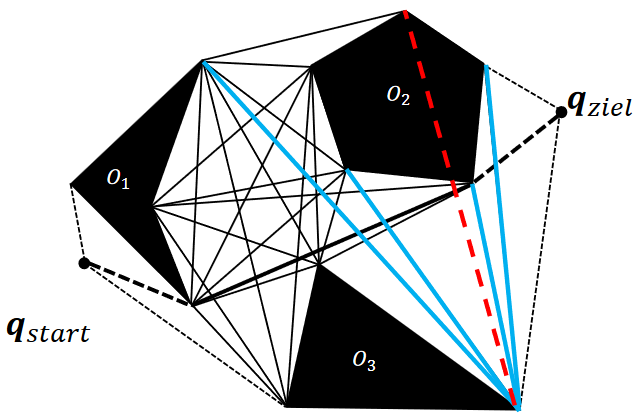
\includegraphics[width=0.4\textwidth]{images/sichtgraph.png}
	\end{center}
	\item \textbf{Vorteile}: Gefundene Weg ist optimal bei 2D-Problemen
	\item \textbf{Nachteile}: Wege sind nicht zwingend kollisionsfrei, da Hinderniskanten auch Wegsegmente sein können $\rightarrow$ \textbf{Lösung}: Erweiterung der Hindernisse
\end{itemize}
\bigskip
\textbf{Zellzerlegung}:
\begin{enumerate}
	\item Zerlege $C_\text{free}$ in Zellen, so dass ein Weg zwischen zwei Konfigurationen innerhalb einer Zelle leicht zu finden ist
	\item Stelle die Nachbarschaft in einem Graphen dar
	\item Suche den optimalen Weg von $\mathbf{q}_\text{Start}$ nach $\mathbf{q}_\text{Ziel}$ in dem Graphen
\end{enumerate}

\textbf{Exakte Zellzerlegung}:
\begin{center}
	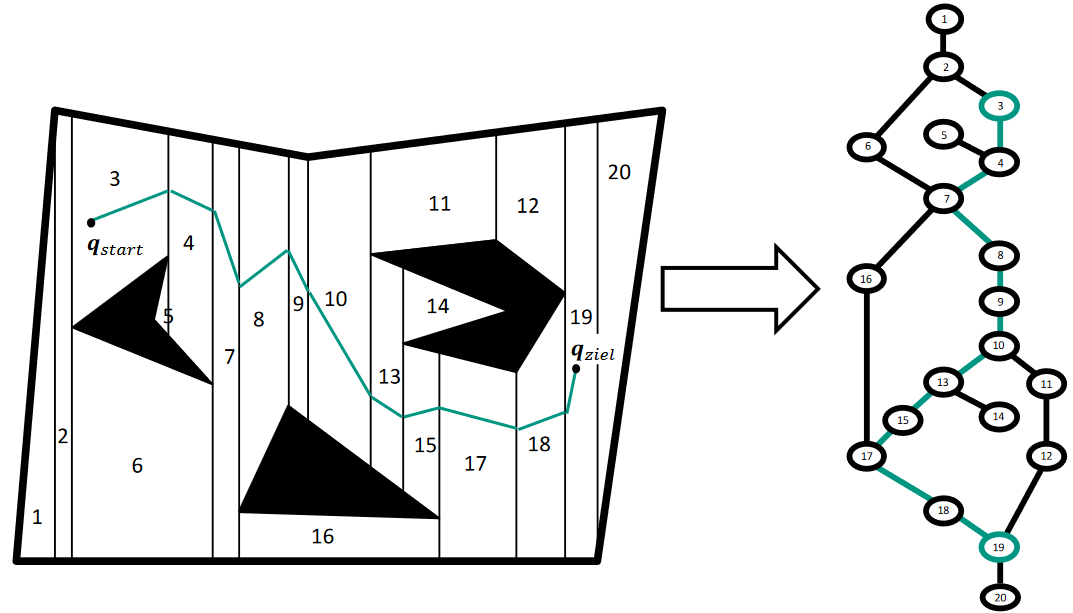
\includegraphics[width=0.7\textwidth]{images/e-zz.png}
\end{center}
\pagebreak

\textbf{Approximative Zellzerlegung}:
\begin{center}
	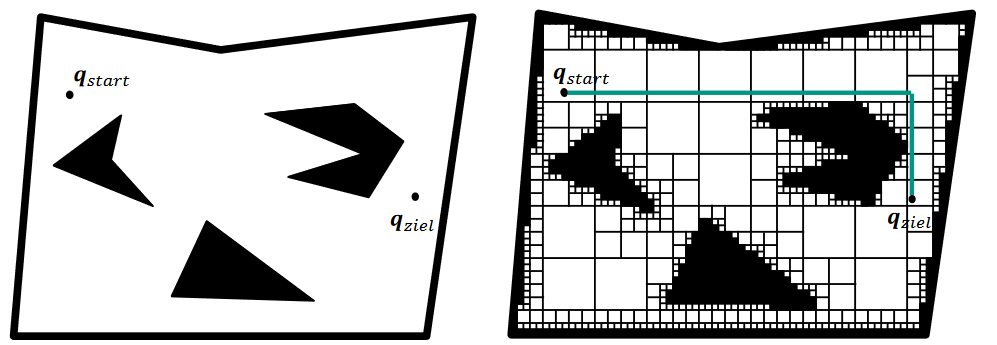
\includegraphics[width=0.7\textwidth]{images/a-zz.png}
\end{center}
\begin{itemize}
	\item \textbf{Vorteil}: Einfache Zerlegung und damit einfachere Wegsuche
	\item \textbf{Nachteil}: Freiraum kann i.A. nur annähernd beschrieben werden
\end{itemize}
\bigskip
\textbf{Baumsuche}:
\begin{itemize}
	\item Darstellung des Konfigurationsraums als \textbf{Quadtree}
	\begin{center}
		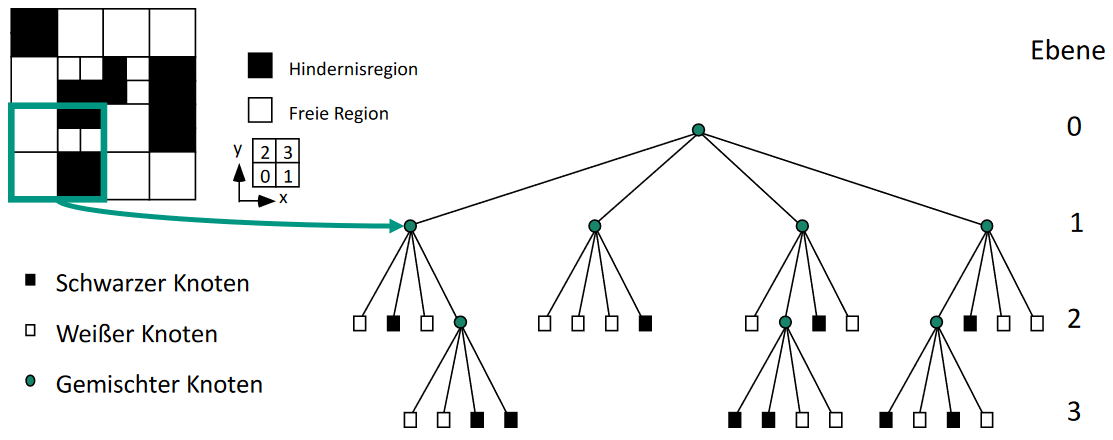
\includegraphics[width=0.7\textwidth]{images/quadtree.png}
	\end{center}
	\item Kacheln finden, in denen sich Start- bzw. Zielkonfiguration befinden
	\item Benachbarte freie Kacheln des Baums vom Start zum Ziel verbinden
\end{itemize}
\bigskip
\textbf{$\mathbf{A^*}$-Algorithmus}:
\begin{itemize}
	\item Liefert kürzesten Pfad von Start nach Ziel
	\item Diskretisiere kontinuierlichen Raum
	\begin{center}
		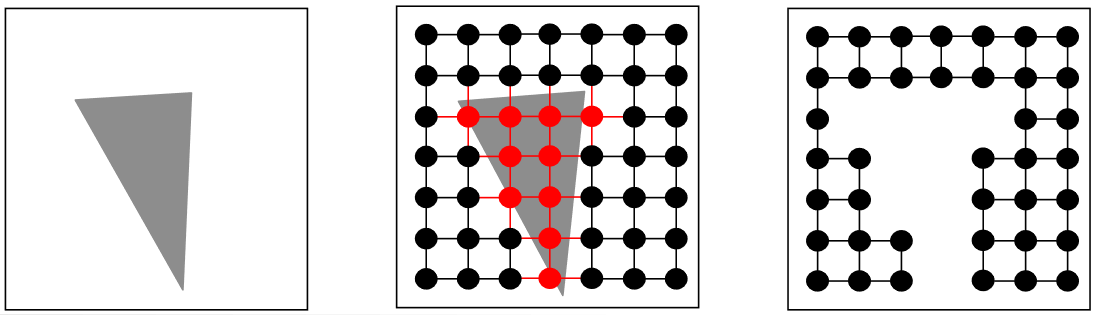
\includegraphics[width=0.4\textwidth]{images/a-s.png}
	\end{center}
	\item \textbf{Kostenfunktion}: $f(x)=g(x)+h(x)$, wobei $g(x)$ Kosten vom Start-Knoten zum Knoten $x$ und $h(x)$ geschätzte Kosten vom $x$ zum Ziel-Knoten entspricht
	\item \textbf{Funktionsweise} ähnlich wie Dijkstra, s. \textit{7/66-76}
	\item Für zulässige Heuristik $h$ ist $A^*$ optimal effizient und findet optimale Lösung
\end{itemize}
\bigskip
\textbf{Potentialfelder}:
\begin{itemize}
	\item Roboter bewegt sich unter dem Einfluss von Kräften, welche ein \textbf{Potentialfeld} auf ihn ausübt
	\item \textbf{Potentialfeld} $U$ ist eine Skalarfunktion über dem Freiraum $U\colon C_\text{free}\rightarrow \R$
	\item Kraft in einem Punkt $\mathbf{q}$ ist der negative Gradient $F(\mathbf{q})=-\nabla U(\mathbf{q})$
	\item Hindernisse erzeugen ein abstoßendes Potential, $\mathbf{q_\text{Ziel}}$ ein anziehendes Potential $\rightarrow$ $\mathbf{q}_\text{Ziel}$ soll das einzige Minimum sein
	\item \textbf{Potentialfunktion}: \textit{7/82-85}
	\item Für das Potential- und Kräftefeld gilt: $U(\mathbf{q})=U_{an}(\mathbf{q})+U_{ab}(\mathbf{q})$ und $F(\mathbf{q})=F_{an}(\mathbf{q})+F_{ab}(\mathbf{q})$
	\begin{center}
		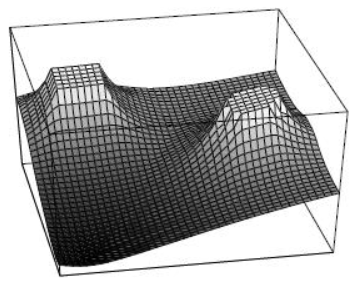
\includegraphics[width=0.2\textwidth]{images/potfeld.png}
	\end{center}
	\item \textbf{Idee}: Roboter läuft entlang eines Tals zum Ziel
\end{itemize}
\bigskip
Nun folgen Algorithmen für \textbf{Bewegungsplanung für Manipulatoren}.

\textbf{Probabilistic Roadmaps}:
\begin{itemize}
	\item Approximation des Freiraumes durch einen Graphen (\textbf{Roadmap})
	\item \textbf{Schritt 1}: Erzeugung eines kollisionsfreien Graphen durch Wählen zufälliger Punkte (\textbf{Sampling})
	\begin{itemize}
		\item Mit \textbf{lokalen Planer} wird überprüft, ob benachbarte Punkte miteinander verbunden werden können
	\end{itemize}
	\item \textbf{Schritt 2}: Verbinde $\mathbf{q}_\text{Start}$ und  $\mathbf{q}_\text{Ziel}$ mit dem Graphen und suche einen Weg von $\mathbf{q}_\text{Start}$ nach $\mathbf{q}_\text{Ziel}$ durch den Graphen (z.B. mit $A^*$)
	\begin{center}
		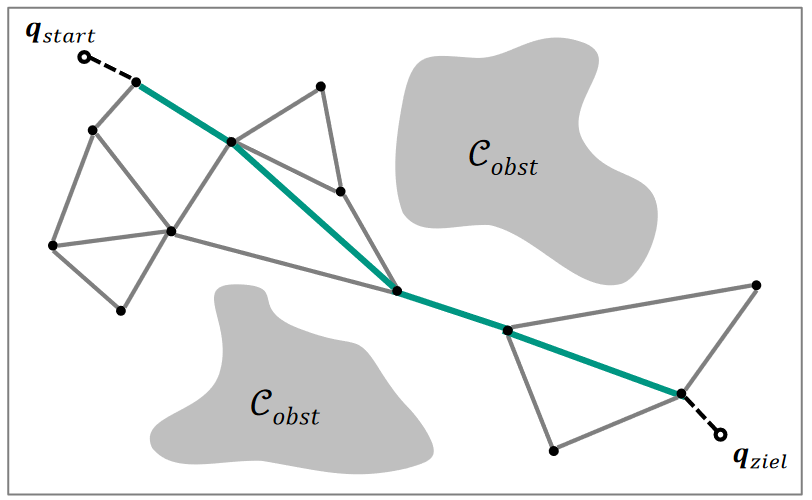
\includegraphics[width=0.4\textwidth]{images/prm.png}
	\end{center}
	\item \textbf{Vorteil}: Sehr gut geeignet für statische Umgebungen, Einmalige Konstruktion des Graphen
	\item \textbf{Probleme}: Hängt stark vom verwendeten Sampling ab, Nicht vollständig, da der Graph den Freiraum nur approximiert
\end{itemize}
\bigskip
\textbf{Dynamic Roadmaps} (DRM):
\begin{itemize}
	\item Approximation des Konfigurationsraums durch eine \textbf{Roadmap}
	\item Approximation des Arbeitsraums durch \textbf{Voxel}
	\item Abbildung $\Phi_{WC}$ von Voxel $\rightarrow$ Roadmap
	\item \textbf{Vorgehen}:
	\begin{enumerate}
		\item Erzeugung einer selbstkollisionsfreien Roadmap durch Wählen zufälliger Punkte (Sampling)
		\item Erzeugung der Abbildung $\Phi_{WC}$ durch Kollisionsüberprüfung zwischen allen Knoten/Kanten und allen Voxeln (sehr rechenaufwändig)
		\item Ermittle alle Voxel mit Hindernis
		\item Lösche alle zugehörigen Kanten und Knoten (mit $\Phi_{WC}$ ermittelt) aus der Roadmap
		\item Verbinde $\mathbf{q}_\text{Start}$ und  $\mathbf{q}_\text{Ziel}$ mit dem Graphen und suche einen Weg von $\mathbf{q}_\text{Start}$ nach $\mathbf{q}_\text{Ziel}$ durch den Graphen
	\end{enumerate}
	\begin{center}
		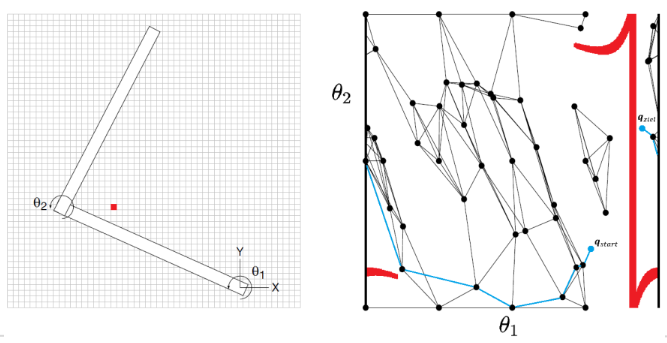
\includegraphics[width=0.6\textwidth]{images/drm.png}
	\end{center}
	\item \textbf{Distance Aware Dynamic Roadmap} (DA-DRM) löscht zusätzlich auch alle Voxel in der Nähe von Hindernissen
\end{itemize}
\bigskip
\textbf{Rapidly-exploring Random Trees} (RRT):
\begin{itemize}
	\item Algorithmus zur Verarbeitung von einmaligen Anfragen, Keine Vorverarbeitung notwendig
	\item Probabilistisch vollständiger, randomisierter Algorithmus
	\item Form von $C_\text{obs}$ im Konfigurationsraum ist unbekannt $\rightarrow$ Kollisionsprüfung im Arbeitsraum
	\pagebreak
	
	\item \textbf{Vorgehen}:
	\begin{enumerate}
		\item Erzeuge leeren Baum $T$ und füge $\mathbf{q}_\text{Start}$ in $T$ ein
		\item Erzeuge einen zufälligen Punkt $\mathbf{q}_S$
		\item Bestimme den nächsten Nachbarn $\mathbf{q}_{nn}$ in $T$
		\item Füge Punkte auf der Verbindung zwischen $\mathbf{q}_S$ und $\mathbf{q}_{nn}$ in $T$ mit Schrittweite $d$ ein, prüfe jeden der Teilpfade auf Kollision und stoppe, wenn eine Kollision erkannt wurde
		\item Gehe zu 2.
	\end{enumerate}
	\item \textbf{Visuelles Beispiel}: \textit{7/109-119}
	\item \textbf{Bidirektionale RRTs}: Baue mit obigem Verfahren 2 Bäume auf, einen von $\mathbf{q}_\text{Start}$ und einen von $\mathbf{q}_\text{Ziel}$ ausgehend. Eine Lösung ist gefunden, wenn beide Bäume mit $\mathbf{q}_S$ verbunden wurden
	\begin{center}
		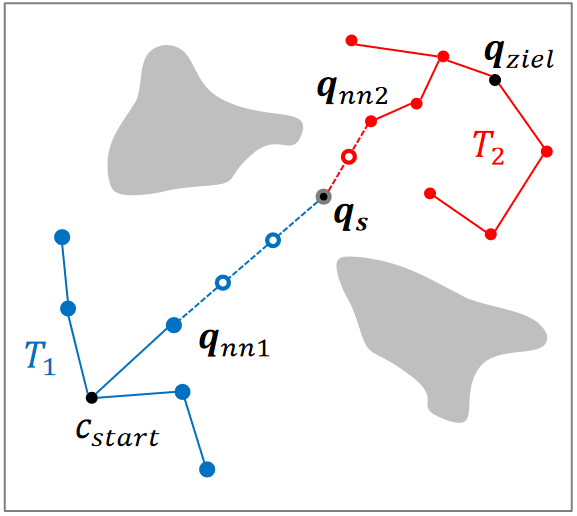
\includegraphics[width=0.3\textwidth]{images/bidirektional-rrt.png}
	\end{center}
	\item \textbf{Nachbearbeitung (Smoothing)}: Falls Verbindung zwischen zwei zufälligen Konten des Lösungsweges kollisionsfrei ist, dann füge Kante zwischen beiden Knoten hinzu und lösche alle dazwischenliegenden Knoten aus dem Lösungspfad $\rightarrow$ Erzeugt glattere Trajektorien
	\begin{center}
		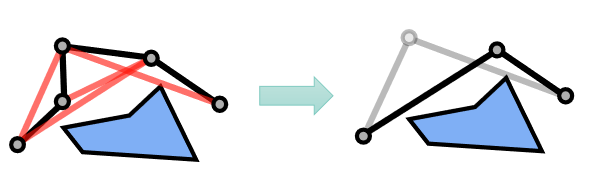
\includegraphics[width=0.3\textwidth]{images/smoothing.png}
	\end{center}
\end{itemize}
\bigskip
\textbf{Constrained RRT}:
\begin{itemize}
	\item Bei der Bewegungsplanung müssen evtl. Nebenbedingungen erfüllt werden
	\item \textbf{Raum der Nebenbedingungen} $C_{NB}\subseteq C$ können niederdimensionale Gebilde im Konfigurationsraum darstellen
	\item \textbf{Idee}: Projiziere eine Stichprobe $\mathbf{q}_S$ auf eine Konfiguration $\mathbf{q'}_S$, die die Nebenbedingung erfüllt
	\pagebreak
	
	\item \textbf{Randomized Gradient Descent}:
	\begin{enumerate}
		\item Zufällige Bestimmung von $n$ Nachbarn von $\mathbf{q}_S$
		\item Falls die Distanz eines Nachbarn zu $C_{NB}$ kleiner als die Distanz von $\mathbf{q}_S$ zu $C_{NB}$, ersetze $\mathbf{q}_S$ mit diesem Nachbarn
		\item Wiederholen bis maximale Iterationszahl erreicht oder die Distanz von $\mathbf{q}_S$ zu $C_{NB}$ kleiner ist als $\alpha$
	\end{enumerate}
	\begin{center}
		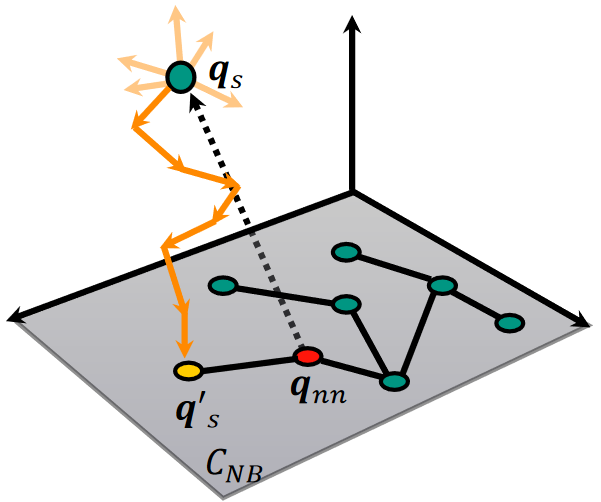
\includegraphics[width=0.3\textwidth]{images/rgd.png}
	\end{center}
	\item \textbf{First Order Retraction}: Berechne $\mathbf{q'}_S$ mithilfe der Jacobi-Matrix
\end{itemize}
\bigskip
\textbf{RRT$\boldsymbol{^*}$}: 
\begin{itemize}
	\item RRT$^*$ optimiert Suchbaum iterativ während der Suche
	\item Optimierung des Suchbaums aufgeteilt in zwei Schritte:
	\begin{enumerate}
		\item Ermittle zu jedem neuen Knoten die Kosten 
		\item Rewiring des Suchbaums beim Hinzugefügen neuer Knoten
		\item Siehe \textit{7/135-138}
	\end{enumerate}
	\item \textbf{Nachteil}: Längere Laufzeiten, Uni-direktionaler Ansatz
\end{itemize}
\bigskip 
\textbf{Enge Passagen}:
\begin{itemize}
	\item \textbf{Problem}: Klassische RRTs können viel Zeit benötigen, bis eine Lösung für einen Durchgang durch eine enge Passage gefunden wird
	\item \textbf{Ideal}: Nur in sichtbarer Voronoi Region eines Knotens sampeln $\rightarrow$ \textbf{Problem}: Berechnung aufwendig $\rightarrow$ Approximation durch Kugel mit Radius $r$ (\textbf{Dynamic Domain})
	\begin{center}
		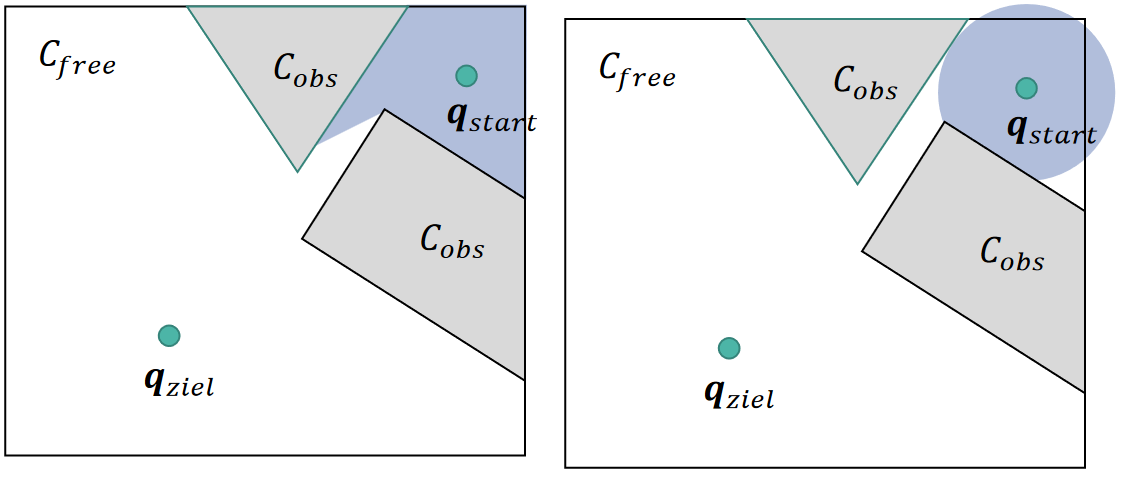
\includegraphics[width=0.6\textwidth]{images/voronoi-sichtbar.png}
	\end{center}
	\item \textbf{Bridge Sampling}: 
	\begin{enumerate}
		\item Wähle gleichverteilt einen zufälligen Punkt $\mathbf{q}_1\in C_\text{obs}$
		\item Wähle nach einer geeigneten Wahrscheinlichkeitsverteilung einen zweiten Punkt $\mathbf{q}_2\in C_\text{obs}$ in der Nähe von $\mathbf{q}_1$
		\item Wenn der Mittelpunkt $\mathbf{q}_S$ zwischen $\mathbf{q}_1$
		und $\mathbf{q}_2$ in $C_\text{free}$ liegt, dann verwende ihn als neue Stichprobe
		\item Wiederhole
	\end{enumerate}
	\begin{center}
		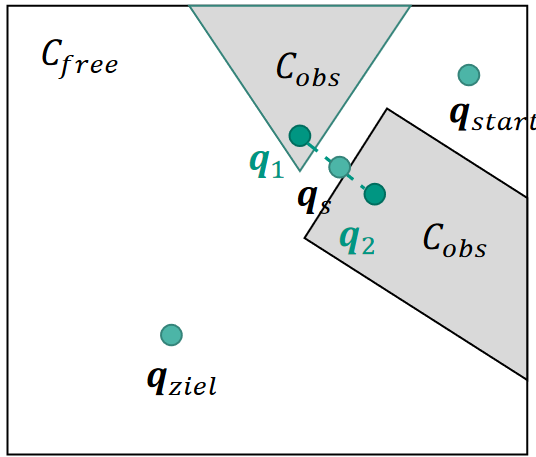
\includegraphics[width=0.3\textwidth]{images/bridge-sampling.png}
	\end{center}
\end{itemize}
